%%%%%%%%%%%%%%%%%%%%%%%%%%%%%%%%%%%%%%%%%%%%%%%%%%%%%%%%%%%%%%%%%%%%
% Grundlagen
%%%%%%%%%%%%%%%%%%%%%%%%%%%%%%%%%%%%%%%%%%%%%%%%%%%%%%%%%%%%%%%%%%%%

\chapter{Material and Methods}
\label{matmet}
\label{lab:matmet:dataset}
To be able to test the following implementations, a dataset containing $93,219$ PSMs was used. Its spectra result from UV-light cross-linked extract from the nucleus of HeLa cells, and these were matched against the nucleus proteins. For each spectrum, up to 4 matching peptides are recorded. The dataset was generated with OpenNuXL~1.0.\\
Of the PSMs, $51,521$ are cross-linked and $41,698$ linear peptides, $50,627$ are target and $42,592$ are decoy peptides. Every PSM has $52$ features, $2$ columns specifying the spectrum and $2$ columns describing the peptide and the protein it originated from, as well as one column indicating to the experimenter whether one entry is a target or a decoy PSM. The features contain the NuXL-score, which was computed from the scores of different algorithms~(see \ref{lab:background:bioinfo_tools}), and was used as a reference.
\renewcommand{\baselinestretch}{0.9}
\begin{figure}
	\normalsize
	\centering
	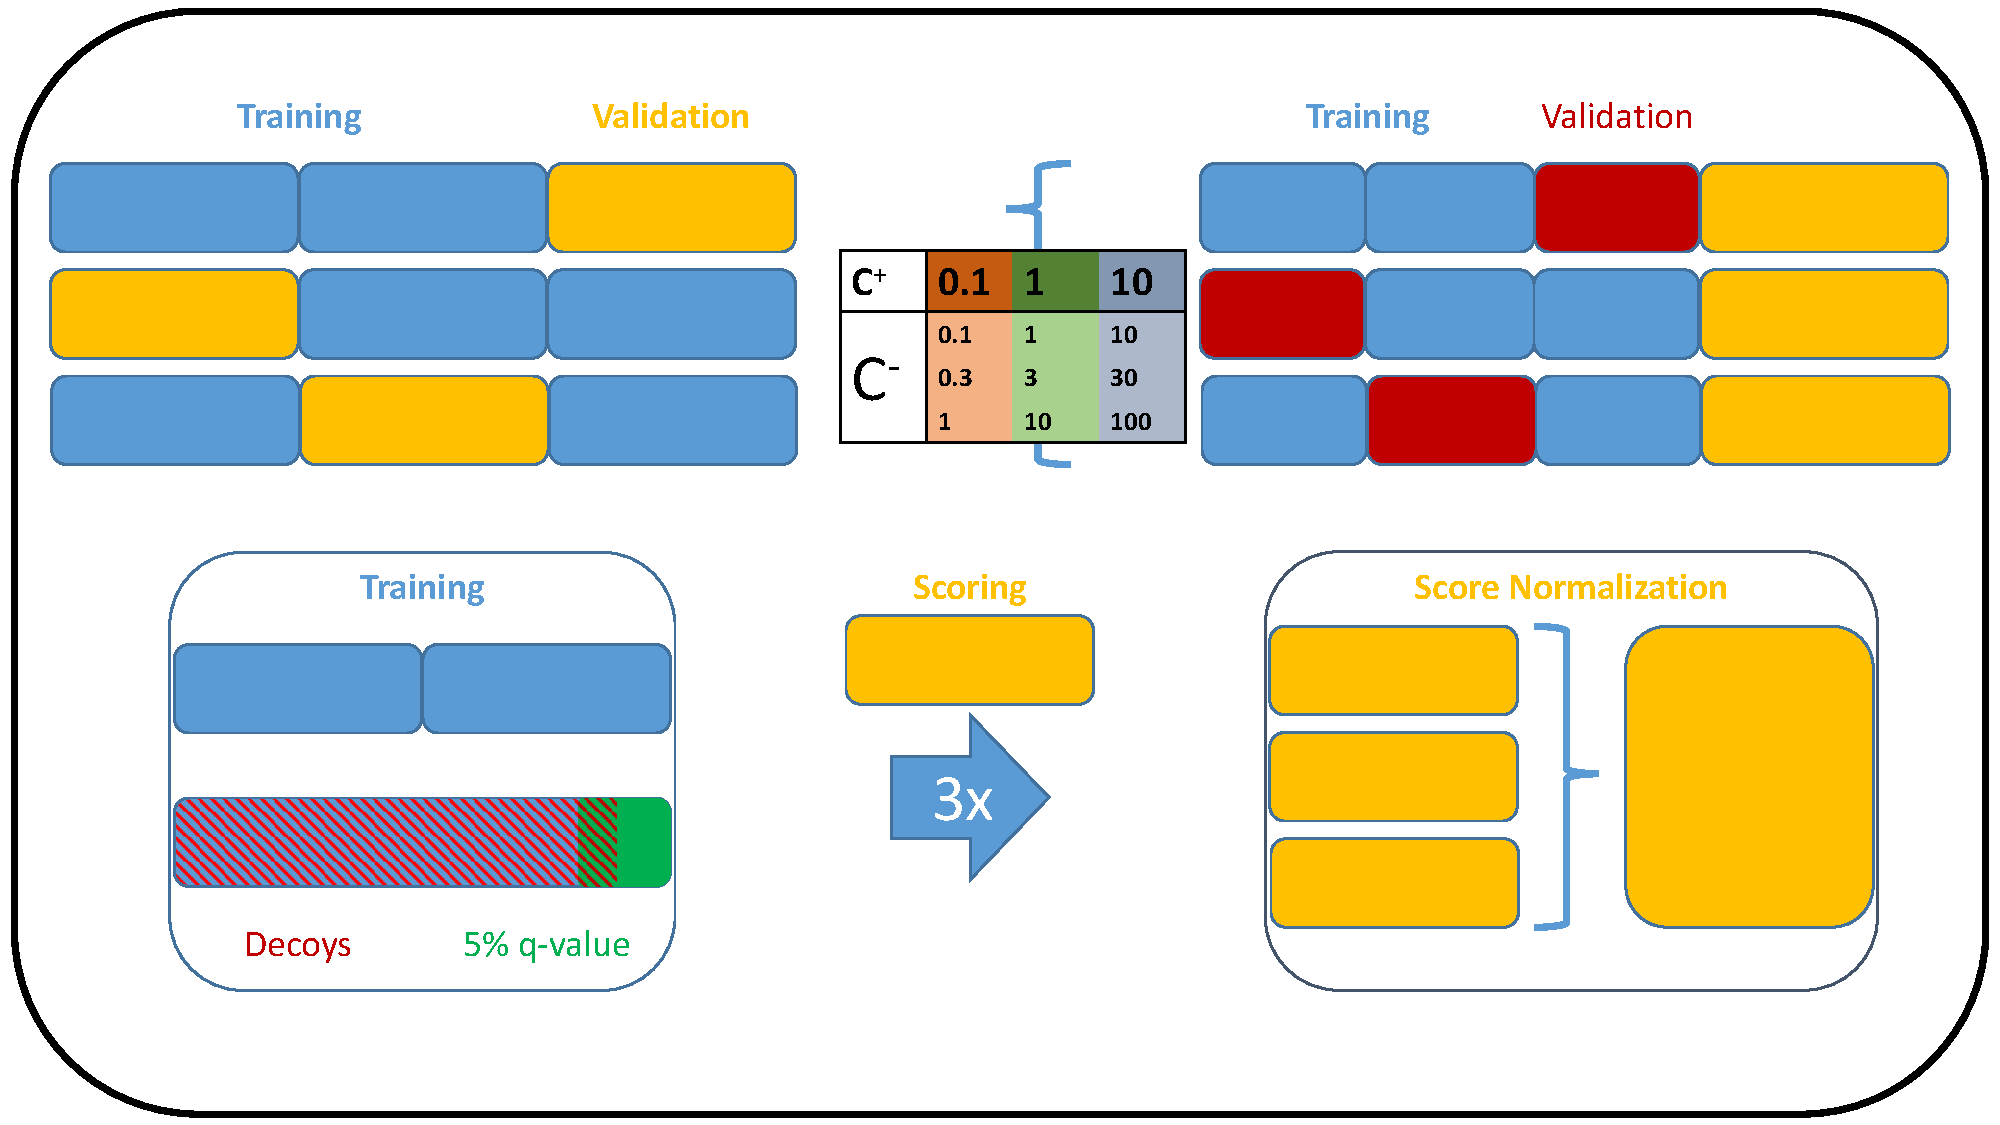
\includegraphics[width = \textwidth]{figures/Percolator_diagram.pdf}
	\caption[Procedure of Percolator]{Rough outline of the Percolator algorithm. First, the dataset is split in three parts, of which two are used for training and one for scoring. Then, another cross-validation is performed on the training part to determine the best parameter combination. Percolator searches the grid spanned by the options for the C parameter for positive examples $C^{+}$ ($0.1$, $1$ and $10$) and negative examples $C^{-}$ ($1$, $3$ or $10 \times C^{+}$). The parameter combination achieving best results on the training set is then used to train an SVM that scores the validation set. For training, all target PSMs with a q-value of $\leq 5\%$ are used as positive and all decoy PSMs are used as negative examples. Because in the end, the dataset will have been scored by three different SVMs, these scores have to be normalized. This is done by a linear transformation mapping the score representing a q-value of $1\%$ to $0$ and the median decoy score to $-1$. If \texttt{qScore} denotes the minimum score for which a q-value of $1\%$ is estimated and \texttt{dMedian} the median score a decoy achieves in the validation set, this sets score is transformed by the following equation: $\text{new Score} = \frac{\text{old score} - \text{\texttt{qScore}}}{\text{\texttt{qScore}} - \text{\texttt{dMedian}}}$.}
	\label{fig:percolator}
\end{figure}
\renewcommand{\baselinestretch}{1}\\

\section{Implementation of the percolator algorithm}
The Percolator algorithm as presented in figure~\ref{fig:percolator} was implemented in python. The pandas\footnote{https://pandas.pydata.org/} package was used for dataset handling, and for SVM calculations and inner cross-validation the classes LinearSVC\footnote{https://scikit-learn.org/stable/modules/generated/sklearn.svm.LinearSVC.html} and GridSearchCV\footnote{https://scikit-learn.org/stable/modules/generated/sklearn.model\_selection.GridSearchCV.html} from the python sklearn package were used. The outer cross-validation was implemented utilizing the numpy array\_split\footnote{https://numpy.org/doc/stable/reference/generated/numpy.array\_split.html} method. An early stopping criterion was implemented, terminating the algorithm if the area under the pseudo ROC curve does not improve over a certain number of iterations. This number is controlled by the parameter \texttt{termWorseIters} and has a default of 4.\\
\label{lab:matmet:normalization}As preprocessing, the provided file is read in as a pandas dataframe (converting strings to floating point or integer values if possible) and q-value and ranks are calculated as discussed in~\ref{lab:background:bioinfo_tools} and~\ref{lab:matmet:ranks} respectively. Also, the columns containing features are normalized. This means, their value is mapped linearly onto $[0,1]$ to avoid rounding errors in features of different orders of magnitude, caused by the representation of floating point numbers.\\
\label{lab:matmet:pseudoROC}For the calculation of pseudo ROC curves and the area under this curve, a function \texttt{pseudoROC} was implemented. It retrieves the entries of the given datasets q-value column, enumerates them and plots the enumeration against the q-values. This results in a pseudo ROC curve. Plotting was performed using the matplotlib.pyplot\footnote{https://matplotlib.org/api/pyplot\_api.html} package, and the area under the pseudo ROC curve was calculated by sklearns auc\footnote{https://scikit-learn.org/stable/modules/generated/sklearn.metrics.auc.html} method.\\
To distinguish the original Percolator algorithm from the version implemented in python and altered here, the latter will be called Pycolator.

\section{Adapting Percolator to Cross-link Identification}
To be able to monitor the difference any experiment makes, especially with respect to the cross-linked or non-cross-linked PSMs, following features were implemented:\\
First, in addition to the q-value, which is calculated as described in~\ref{background}, the calculation of a class-specific q-value was implemented. This is done by splitting the dataset according to the class affiliation and calculating the q-value separately for both splits. This allows a more precise performance estimation when looking at only one of the classes.\\
\label{lab:matmet:rocs_after_every_iteration}
Second, a ROC curve using the \texttt{pseudoROC} function~(\ref{lab:matmet:pseudoROC}) is plotted after every iteration of Pycolator: one for the whole dataset, one only for cross-linked, and one only for non-cross-linked PSMs. Accordingly, the respective class-specific q-value is used. Thus, three plots covering the corresponding class(es) and every iteration, as well as the area under the curve are output. This allows for fast visual detection of the impact a specific change to the algorithm has on certain classes, iterations or general sensitivity.
\subsection{Different Ranks}
\label{lab:matmet:ranks}
As experience shows, cross-linked peptides can be harder to detect than linear peptides. This means, the possibly correct cross-linked peptide will frequently not get the highest score of all the peptides. It thus can be beneficial to not only consider the highest scoring peptide, but also the highest scoring cross-linked peptide or also some lower-scoring peptides, and assign them ranks. Then, as following experiments show, Percolator can correct the scores of some lower-ranking PSMs, possibly detecting more cross-linked PSMs. Meanwhile it is known to the experimenter, that only one of the peptides can be the correct match to a spectrum, and thus any PSM with a lower rank than 1 should be excluded at the end.\\
To tackle both constraints, Pycolator first trains the SVM with every PSM available and re-calculates the ranks based upon the newly assigned score after every iteration, possibly correcting the ranks of some PSMs. When the used metric, normally the area under the pseudo ROC curve, does not improve beyond a certain threshold per iteration, every PSM with rank $2+$ is dropped. The threshold is controlled by the parameter \texttt{cutOffImprove} with a default of $0.01$ corresponding to a $1\%$ increase of the used metric per iteration. Since also some of the best scoring PSMs will be dropped (even though they were not assigned rank 1), the algorithm then runs further until the maximum iterations are reached or the score does not further improve, in order to properly integrate and score the new PSMs considered confident.\\
The performance of this feature was tested against dropping the lower ranking PSMs once at the very end of the algorithm and once at the very beginning. Pycolator was run on the given dataset~(\ref{lab:matmet:dataset}) and pseudo ROCs were plotted as described in~\ref{lab:matmet:rocs_after_every_iteration}.
\subsection{Characteristics of Cross-linked PSMs}
Apart from being hard to detect, cross-linked peptides also have other characteristics, some of which pose problems to the computational detection of correct PSMs. As discussed in~\ref{lab:matmet:splitting}~"Splitting the dataset", the features of cross-linked and linear peptides are so dissimilar, splitting the dataset and training a linear SVM separately on cross-links and non-cross-links yields significantly better results than training one linear SVM. To reduce the impact of this heterogeneity, the following experiments were conducted:
\subsubsection{Proportions of Different Classes}
\label{lab:matmet:proportions}
As discussed in~\ref{lab:background:percolator}, Percolator employs a nested cross-validation approach, splitting the dataset, training on all parts than one and testing/scoring on the remaining part. If the splitting was uneven by chance, the SVM would be trained badly and the scoring inaccurate. Having different classes with significant differences in the dataset, like in our case cross-linked and linear PSMs or targets and decoys, increases this problem. For example, if there was a testing split with many cross-linked PSMs, the SVM had to be trained on the remaining data with few cross-linked PSMs, resulting in probably poor scoring of the many cross-linked PSMs in the test set. In the average case, this should not be a problem, but it can occasionally produce worse or better results, which would follow from overfitting.\\
To solve this problem, a mechanism of maintaining the proportion of the classes in the whole dataset for every inner and outer split was implemented. It can be toggled for targets and decoys or cross-linked and non-cross-linked PSMs as well as for inner and outer split independently. The impact has been measured by running the algorithm $10$ times, plotting and recording the results of the best, worst and median run w.r.t. to the q-value any number of PSMs was identified at. Because this took approximately 90 minutes, the test was performed in a Google Colaboratory notebook\footnote{The Google Colaboratory notebook used:\\ \url{https://colab.research.google.com/drive/1VqZAmdta57YhgobA0WkQMqe_U9YIUnDl?usp=sharing}}.
%\begin{figure}
%	\label{fig:fluctuation_of_percolator}
%	\centering
%	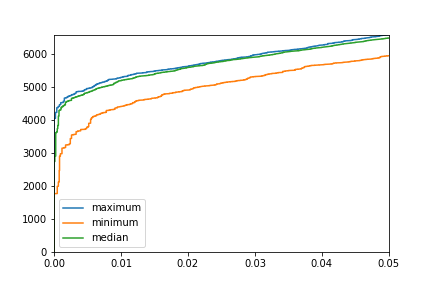
\includegraphics[width = 0.7\textwidth]{figures/percolator_MaxMinMedian_ClassesOption=.png}
%	\caption[Fluctuation of an earlier version of Percolator]{Pseudo ROC curve of an earlier version of the Percolator algorithm. It was run $10$ times and the best, worst and median run were plotted. Although the best run is close to the median one, the worst run is off by almost $1000$ PSMs. }
%\end{figure}
\subsubsection{Imputation}
\label{lab:matmet:imputation}
Cross-linked PSMs naturally have features linear PSMs do not have, which can however be used for training the SVM. An example would be the nucleotide it was linked to, or the partial loss score, which is the X!~Tandem~\cite{Craig2004} hyper score for the cross-linked peaks. In the given dataset~(\ref{lab:matmet:dataset}), $16$ out of $61$ features were only given for cross-linked PSMs. Optimally, these should not influence the score a non-cross-linked PSM gets. However, $0$ was filled in for the missing values and because that is a valid value for the linear SVM, it biases the decision made. For example, if a high value in a feature leads the SVM to a decision against the PSM, $0$ as the lowest value possible after feature normalization~(\ref{lab:matmet:normalization}) will tell the SVM to give the PSM a higher score. The procedure of replacing missing values with numbers minimizing the bias is called imputation. The scikit-learn package provides methods for the implementation in python\footnote{https://scikit-learn.org/stable/modules/impute.html}, and one of these, the \texttt{IterativeImputer}~function, was tested.
\subsubsection{Splitting the Dataset}
\label{lab:matmet:splitting}
Because the SVM is linear, one feature can not alter the influence another feature has on the decision. Thus, splitting the dataset into cross-linked and non-cross-linked PSMs should allow the SVM to fit more precisely onto the characteristics of each. This was tested by running Pycolator on each split and the concatenate the datasets, recalculating the q-values from the Pycolator scores. It was also tested splitting the dataset by the nucleotide the peptide was cross-linked onto, and non-cross-linked PSMs as a fifth class.
\subsection{Small datasets}
\label{lab:matmet:small_datasets}
The portion of cross-linked peptides in a dataset is often very small. To evaluate when splitting as proposed in~\ref{lab:matmet:splitting}~"Splitting the Dataset" is possible and obtain general insight into the scalability of Pycolator, two experiments were conducted to conclude how small a dataset may be, so that the Percolator algorithm still works. In each case, Pycolator was applied to a dataset sampled from the given one~(\ref{lab:matmet:dataset}). The area under the pseudo ROC curve and the number of PSMs identified at $1\%$ q-value were recorded and used as metrics. The results achieved by Pycolator were compared to the effect the splitting had on the q-value estimation utilizing the given, precomputed NuXL score.\\
First, the smaller dataset was sampled using every $2^i$-th PSM from the whole dataset with $i\in\mathbb{N} \land i\in[0,13]$. Second, the smaller dataset was sampled randomly using a uniform distribution from all PSMs with a q-value of $<10\%$. The portions sampled were $\frac{1}{2^i} : i\in\mathbb{N} \land i\in[0,12]$. Additionally to the metrics mentioned above, also the expected number of identifications at $1\%$~q-value for each split were calculated and recorded. This was done by counting the number of such PSMs before re-estimating the q-value or letting Pycolator run, thus being the number of identifications by the NuXL score if the q-value is estimated based on the whole dataset.
%For the NuXL score as reference and the Pycolator score respectively one plot showing the portion of PSMs with a q-value of $1\%$ and one plot showing the ratio of found to number of expected PSMs with $1\%$ q-value as a function of the dataset size were generated. In the end, the ratio of AUCs and identifications at $1\%$ q-value generated by the NuXL vs Pycolator score were plotted as a function of the dataset size. 
To compensate for the randomness in this experiment, Monte-Carlo-Sampling with 10 iterations was performed and the results are presented with boxplots.\\
Because numerical problems occur when calculating the area under a pseudo ROC curve of a very small dataset (since the curve consists of only one point), another metric was introduced: the number of identified PSMs at a q-value threshold of $1\%$. Per default, Pycolator decides automatically after its first iteration if this metric is required based on the dataset, and adjusts its log, plots per iteration and functions like the early stopping criterion accordingly.\\\\
(- Performance auf anderem Datensatz\\
- Vergleich mit Entrapment FDR)